\subsection{RQ4:How are the security and performance is ensured in
a product of a company?}
\label{RQ4}
This particular question covers how a company secures its code from external attack and maintain its performance after deployment. It also slightly deals with the problem of scalability. Performance depends greatly on whether a product has scalability or not. So, we will cover the following points here:
\begin{itemize}
    \item Security
    \item Performance
    \item Scalability
\end{itemize}
\subsubsection{Security}
\label{Security}
\begin{figure}[htbp]
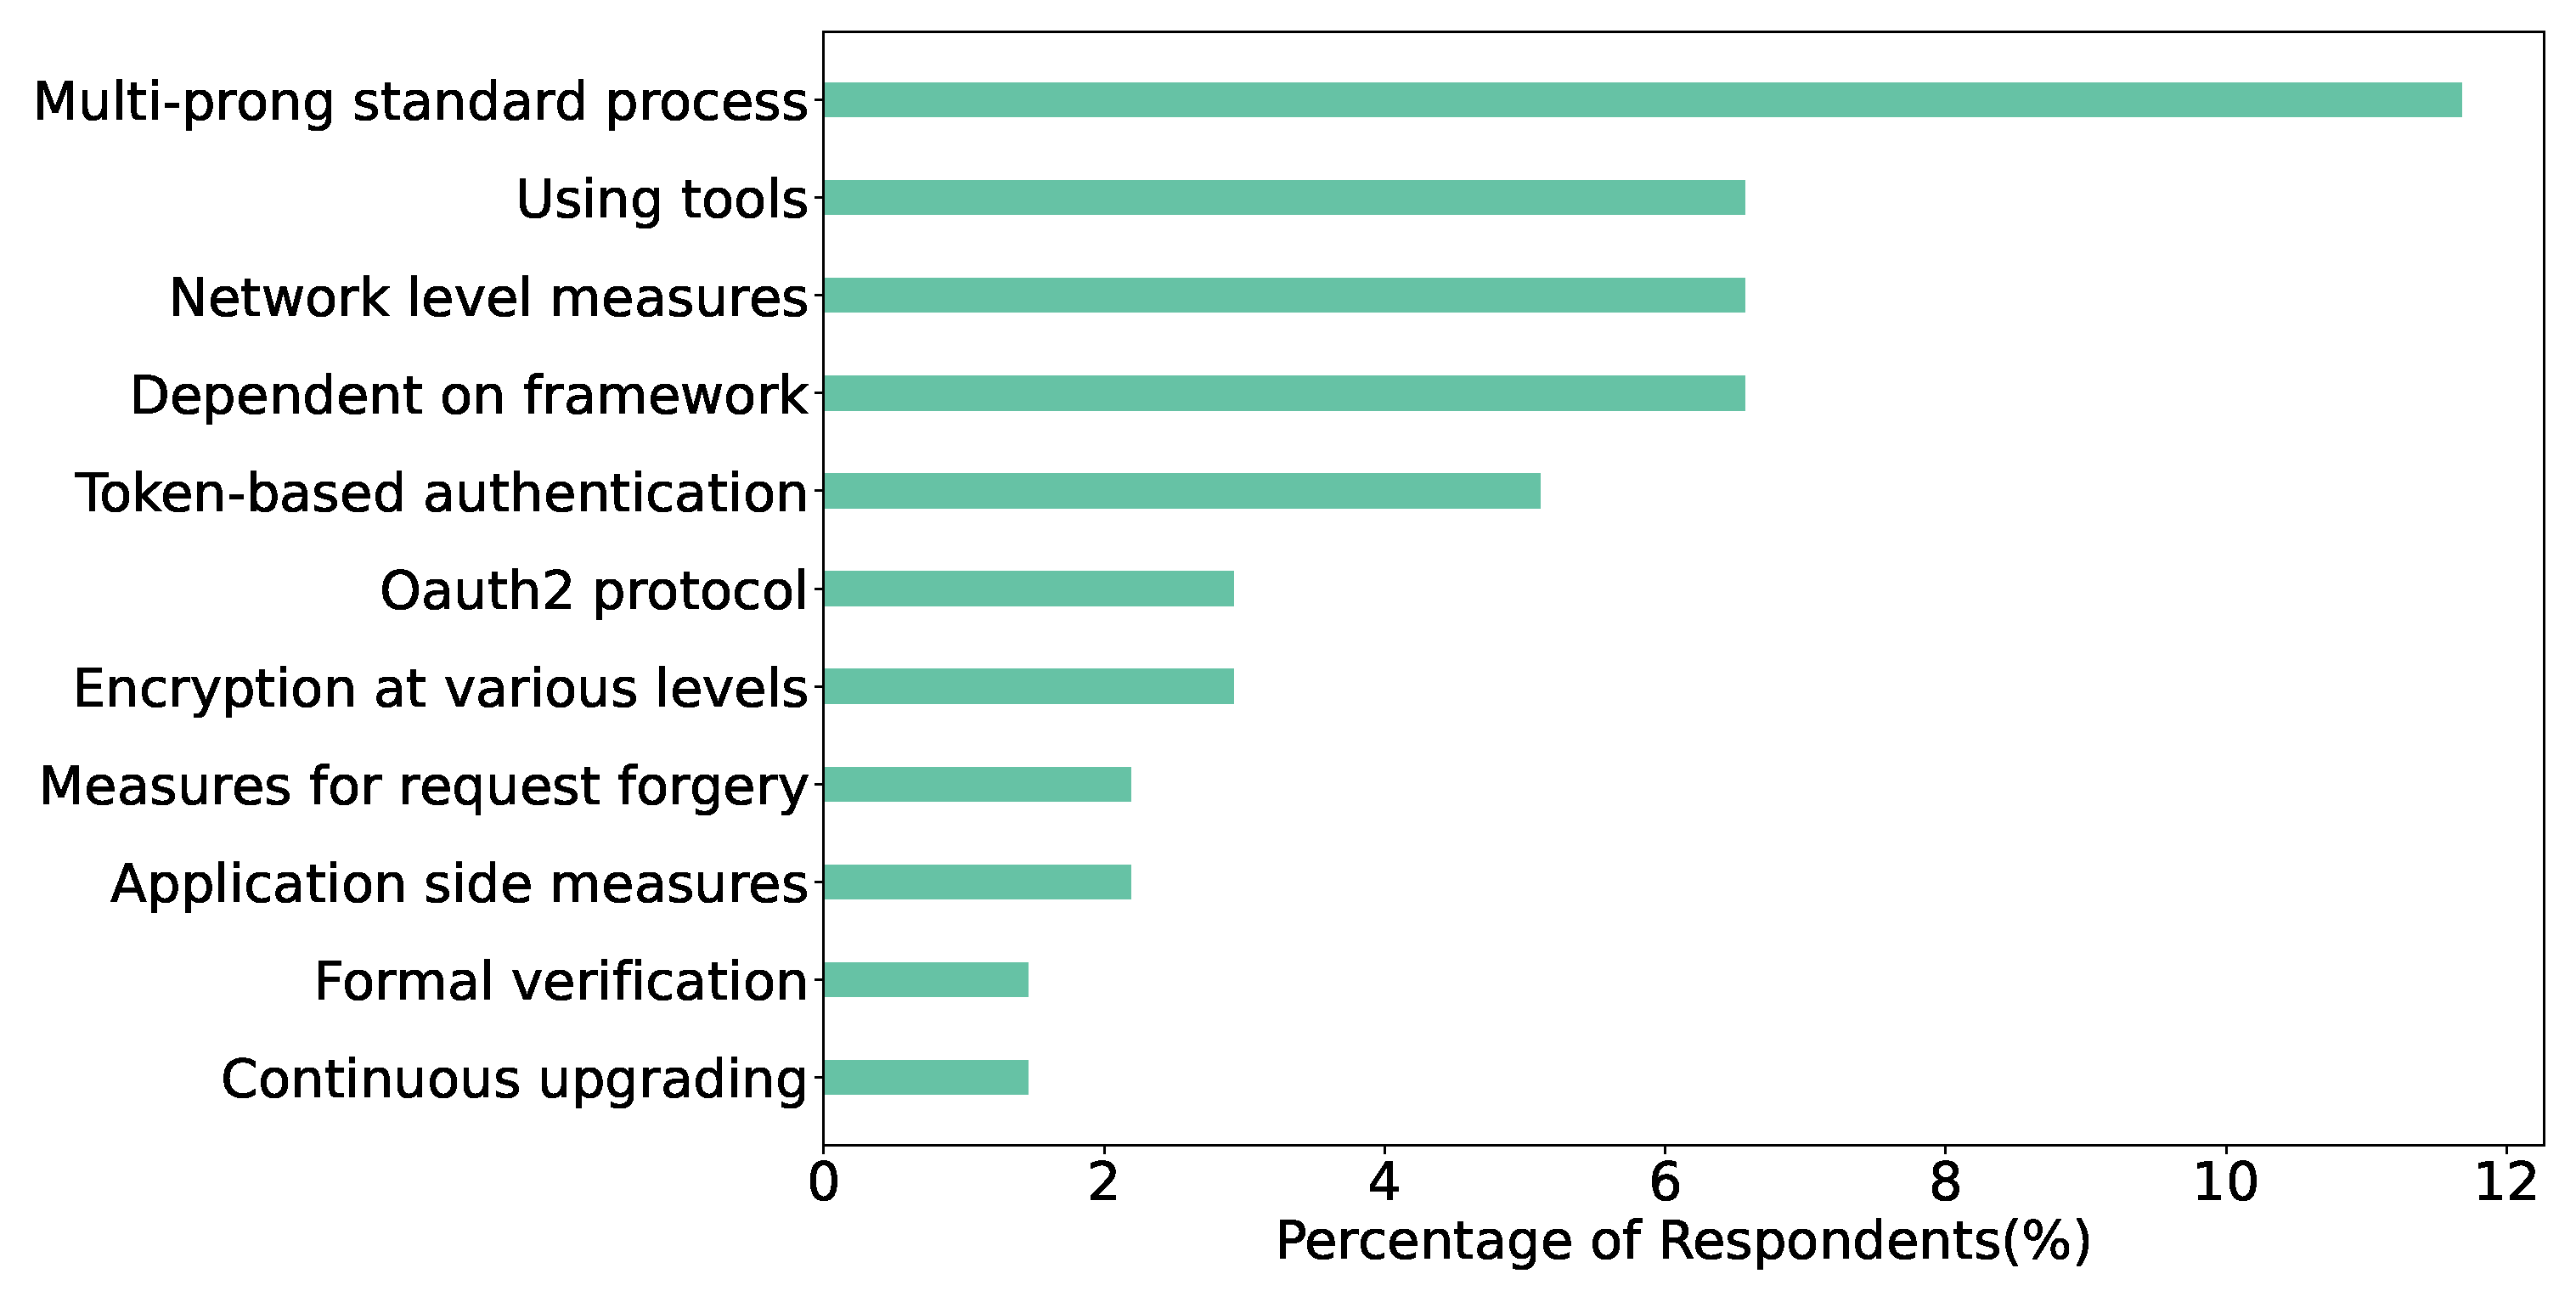
\includegraphics[scale=0.28]{Figures/Security.eps} 
\caption{Measures to maintain security of products}
\label{fig:Measures to ensure security}
\end{figure}
\hfill\\
Security refers to confidentiality, integrity and authenticity. To maintain security of software product SE industry of Bangladesh is mainly dependent on Standard process which includes cloud based security, third party software, OS hardening followed by uses of security tools, network level measures and framework security. As found by Harrison et al.\citep{Harrison2010} network level measures are the first choice in ensuring security of software product which matches with our findings. Srinivasan et al.\citep{Srinivasan2017} listed top 10 web framework in terms of security testing where Spring framework achieved 7\textsuperscript{th} position. From figure ~\ref{fig:frameworks} we have seen that most of our respondents use Spring framework for software development. This might be the reason that a lot number of respondents dependent on framework for ensuring security.
\begin{enumerate}

    \item \textbf{Application Side Measures}: Security is ensured at the software or application side. 2.19\% respondents implemented security measures at application level.
    \surveyquote{At application level, could not achieve others yet}{72}
    
    \item \textbf{Server Side Measures}: Security is ensured at the server side. 0.73\% respondents implemented security measures at server level.
    \surveyquote{We use github/bitbucket repository systems to code maintain and store. We use server side security on AWS and other third party server host.}{48}
    
    \item \textbf{Network level Measures}: Network level measures include IP-white-listing, port-blocking, VPN and  use of HTTPS  in software. 6.57\% respondents use at least one of the before mentioned strategy to ensure security.
    \surveyquote{network blocking and common security measures}{2}
    
    \item \textbf{Formal Verification}: Security threats can be mitigated by  a code level review . 1.46\% respondents ensured the practice of formal code review
    \surveyquote{There are some basic guidelines that we must follow and while code review this needs to be an absolute part that needs to be checked before the code gets merged}{112}
    
    \item \textbf{Measures for request forgery}: Measures against cross site forgery is implemented to ensure security. This includes CORS or cross origin resource sharing, CSRF or cross site request forgery or one click attack or XSRF. 2.19\% respondents implemented measures agianst  Cross-site request forgery to ensure security.
    \surveyquote{Security testings like: SQL injection, cross-site scripting, CSRF, API security, use of https,  detecting malicious / suspicious HTTP requests and auto-blocking}{42}

    \item \textbf{OAuth 2.0} : OAuth 2.0 is the industry-standard protocol for authorization. OAuth 2.0 focuses on client developer simplicity while providing specific authorization flows for web applications, desktop applications, mobile phones, and living room devices. Many (2.92\%) respondents use OAuth 2.0 protocol as the main way of maintaining security.
    \surveyquote{OAuth 2.0, JWT, Token Base Authentication, CORS Filter, XSRF}{127}
    
    \item \textbf{Token-based authentication} : A token-based authentication system allows users to enter their username and password in order to obtain a token which allows them to fetch a specific resource - without using their username and password. Once their token has been obtained, the user can offer the token which offers access to a specific resource for a time period - to the remote site. 5.11\% people expressed its eligibility.
    \surveyquote{Token based authentication for all of my rest service}{80}
    
    \item \textbf{Multi-prong Standard Process} : Following multiprong standard processes is the best way to enforce security. About 10.22\% of the total respondents expressed this opinion.
    \surveyquote{Multi Prong Standard Processes and Products}{110}
    
    
    \item \textbf{Encryption at Various Levels} : Not only at password,but also in every level of software, encryption is first and foremost to ensure its security.
    \surveyquote{use encryption at different level of software (server, network, transmission layer, database and software layer.)}{35}
    
    \item \textbf{Use of tools} : Respondents use various open-source/ paid tools for scanning  and testing. These tools help to find security threats in an existing system. The tools includes OWASP based tools and  penetration testing tools
    \surveyquote{use encryption at different level of software (server, network, transmission layer, database and software layer.)}{35}
    
    
    \item \textbf{Dependent on Framework} : Common framework provides basic to intermediate level security measures in the application. 6.57\% respondents depends on framework for security. The framework includes spring and  HDIV.
    \surveyquote{https, popular framework which already prevents some type of attacks. rest of the things on case-by-case basis)}{79}
    
    
    \item \textbf{Non-disclosure agreement} : 2.19\% refused to provide any details due to non-disclosure agreement.
    \surveyquote{As we are regulated by Bangladesh Bank as a payment processing platform, we need to maintain certain security compliance which cannot be disclosed here. The security compliance is similar to the PCI DSS compliance which I can say}{10}
    
    \item \textbf{Continuous Upgrading}: As security threats are evolving thus current systems need continuous upgradation in a frequent interval. 1.46\% respondents said they arrange frequent hackathon, workshop, security audits to address the continuously evolving security threat.
    \surveyquote{We run security audit of our office environment. We also conduct security session per 6 months to introduce latest trend in threats and what we can do to avoid it}{57}
    

   
\end{enumerate}

\subsubsection{Performance}
\label{Performance}
\begin{figure}[htbp]
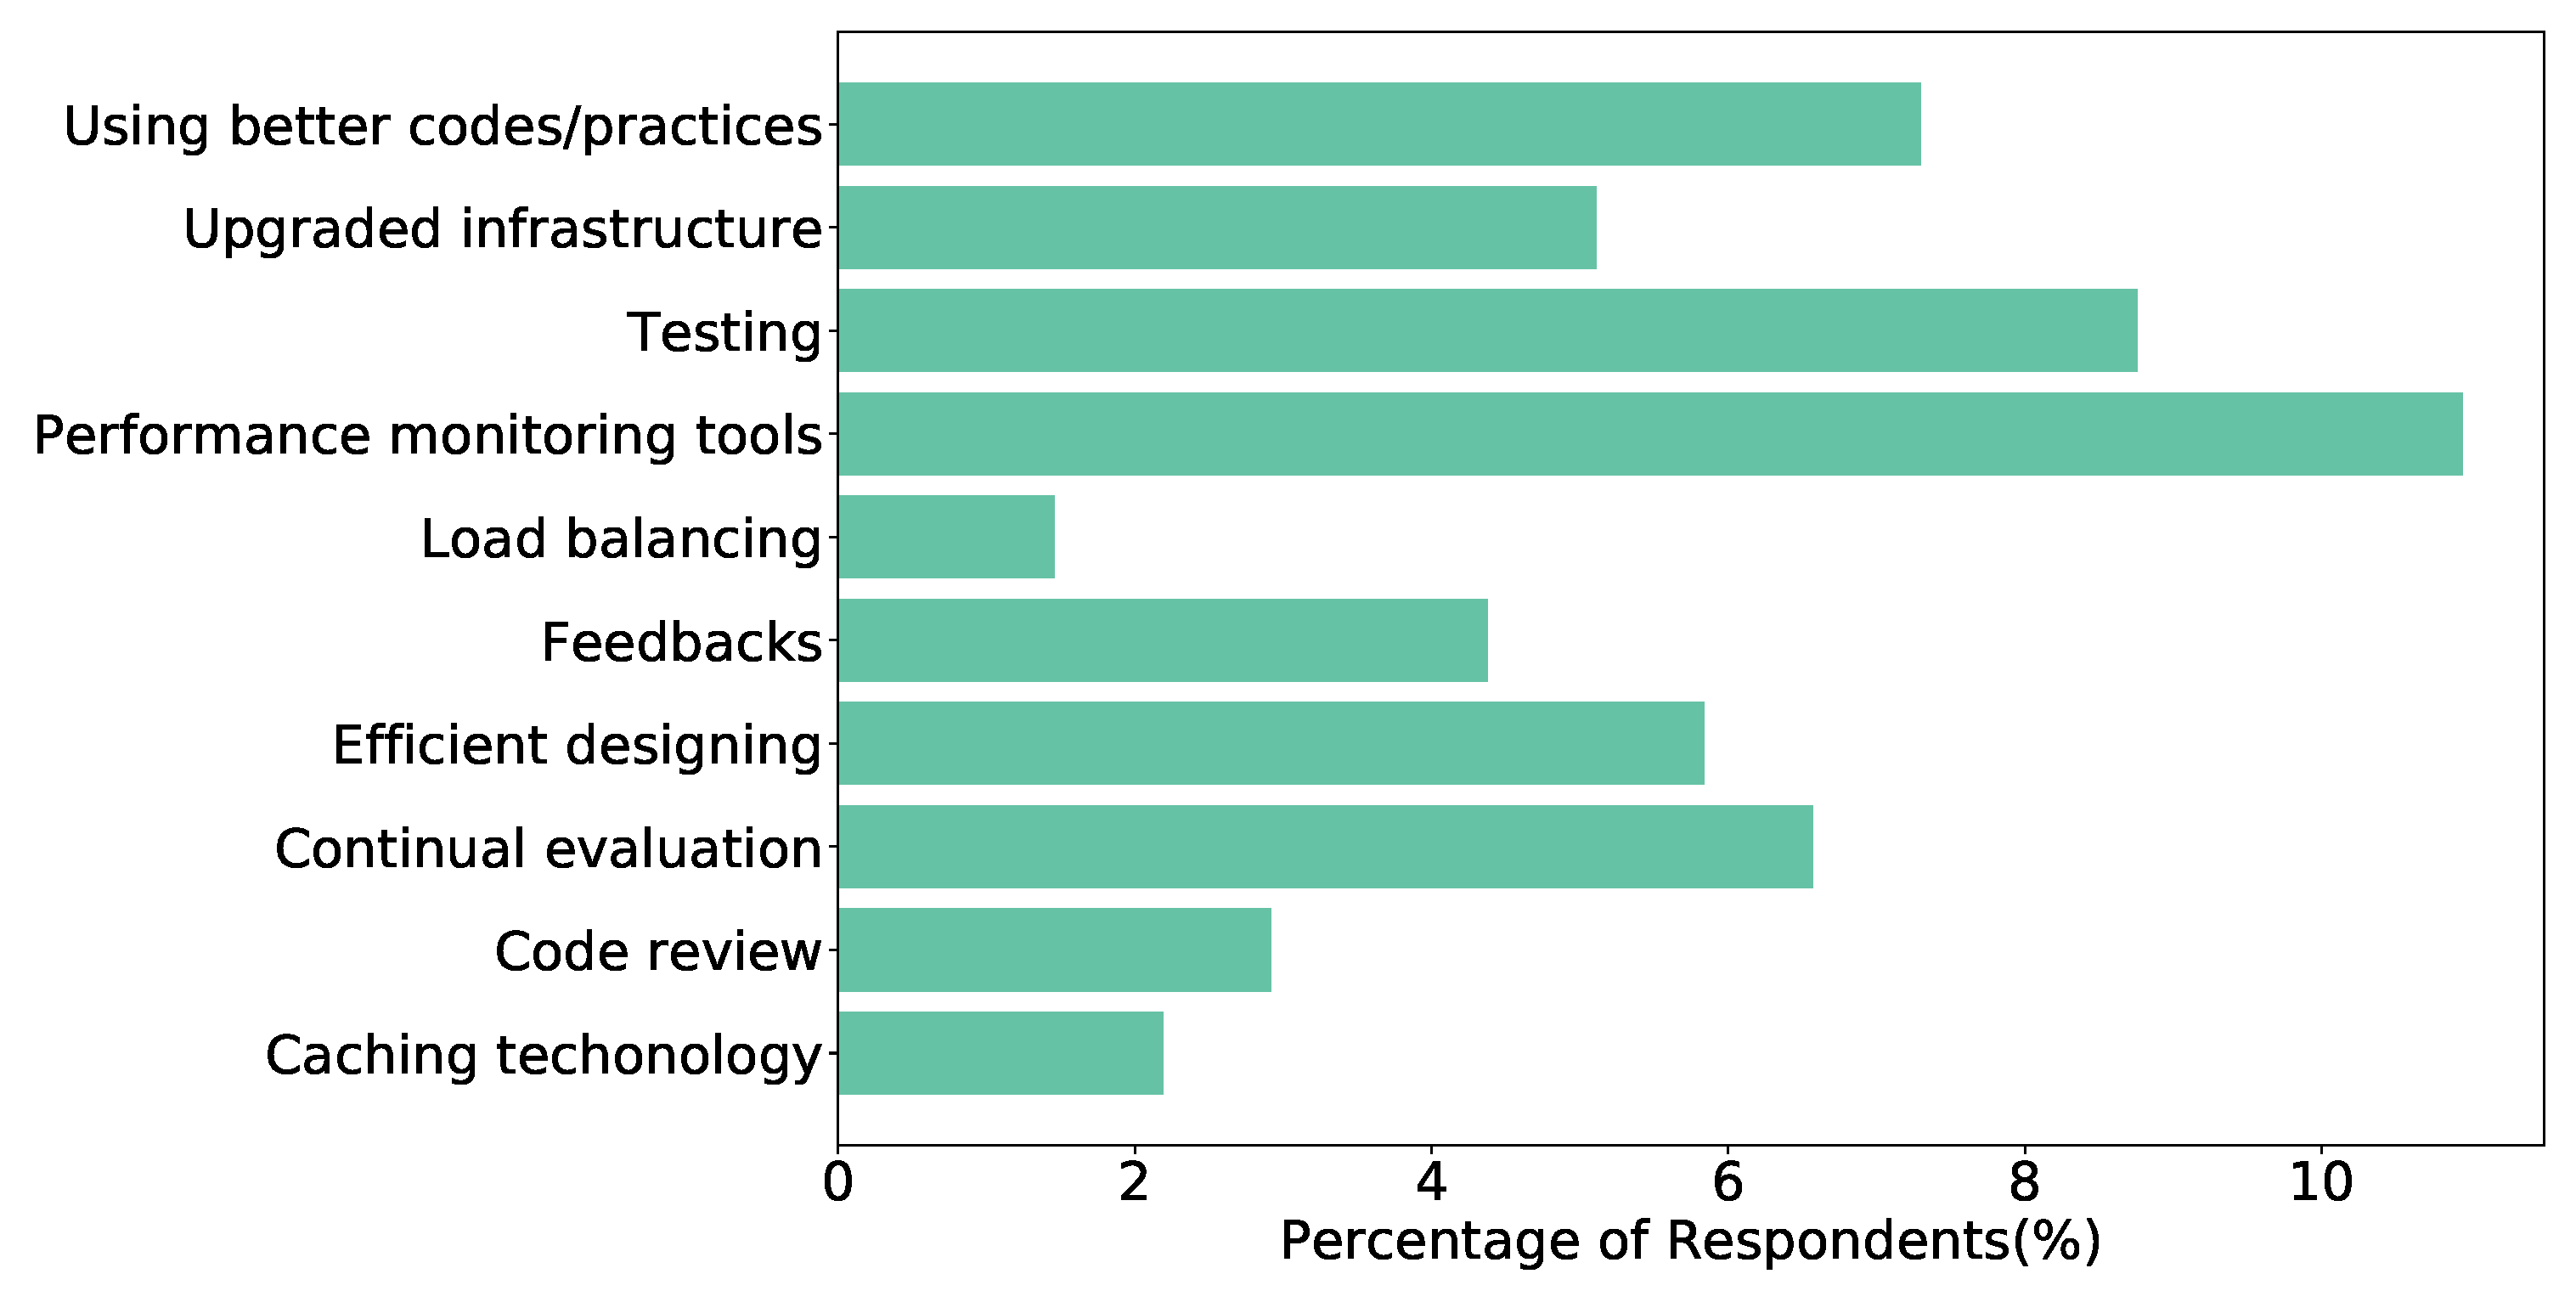
\includegraphics[scale=0.28]{Figures/Performance.eps} 
\caption{Measures to ensure performance of products}
\label{fig:Measures to ensure performance}
\end{figure}
\hfill\\
Software performance indicates how efficient the software is in terms if resource and time. Testing tools such as load testing are common measure\citep{Liu2009} to ensure performance of a software on this regard Bangladesh SE industry follows the same measures. According to our respondents the top three performance ensuring method in Bangladesh SE industry is use of tools, test and better codes/practices or design-implementation level measures. 
\begin{enumerate}

    \item \textbf{Caching Mechanism}: Caching mechanism improves performance by reducing response time. 
    \surveyquote{... Good Caching}{29}
    
    
    \item \textbf{Emphasize on design}: Software performance is dependent on architecture of system. 5.84\% respondents emphasize on design to ensure performance.
    \surveyquote{By careful designing}{24}
    
    
    \item \textbf{Testing}: Performance is ensured by various rigorous testing phase. The phase includes load testing, stress testing, integration testing.
    \surveyquote{By rigorous testing and checking performance testing}{17}
    
    
    \item \textbf{Emphasize on Infrastructure}: 5.11\% respondents use upgraded infrastructure to ensure performance. These infrastructure includes cloud hosting, high end server, new technologies.
    \surveyquote{Amazon Hosting and Quality Software}{85}
    
    
    \item \textbf{Implementing best practices}: Industry standard best practices can improve system performance. 7.3\%respondents ensure performance by implementing best practices. The best practices include compression technology, enforcing design patterns and refactoring.
    \surveyquote{Implementation time carefulness and maintaining a well developed coding standard}{40}
    
    
    \item \textbf{Load Balancing}: Load balancing can improve the system performance by ensuring equal load to all servers. 27.1\% respondents think of using load balancing as a measure to maintain performance.
    \surveyquote{Optimizing number of HTTP requests, Asynchronous programming, Caching, CDN, Load Balancing, nginx, varnish, compression of data, Continuous monitoring, Load testing, stress testing}{42}
    
    \item \textbf{Performance Monitoring Tools}: There are various performance monitoring automated tools from which we can measure the overall as well as component-wise performance of a product. 10.95\% respondents use these tools to measure performance.
    \surveyquote{take help of different performance monitoring tools and dashboard, analyzed data , measure time and memory efficiency of process}{35}
    
    \item \textbf{User Feedback}: It is a great source of performance measure. Taking a time to time feedback from the clients help a company to realise how their products are performing actually. Many (4.38\%) respondents have highly recommended it.
    \surveyquote{Continuous feedback from clients and QA team}{65}
    
    \item \textbf{Continual Evaluation}: If there are some problems about performance, it can easily be identified in continuous monitoring and evaluation of the products. 6.57\% of the total respondents have thought of this as a better solution.
    \surveyquote{regular rechecking/running of automation scripts as a automation tester}{14}
    
    \item \textbf{Code Review}: About 2.92\% people have said that a proper and attentive code review can reduce the faults in the codes and therefore enhance the performance of a software.
    \surveyquote{The code quality is assessed by the different team members during code review, followed by designing new ways to solve issues in the product that are time-intensive.}{15}
\end{enumerate}

\subsubsection{Scalability}
\label{Scalability}
\begin{figure}[htbp]
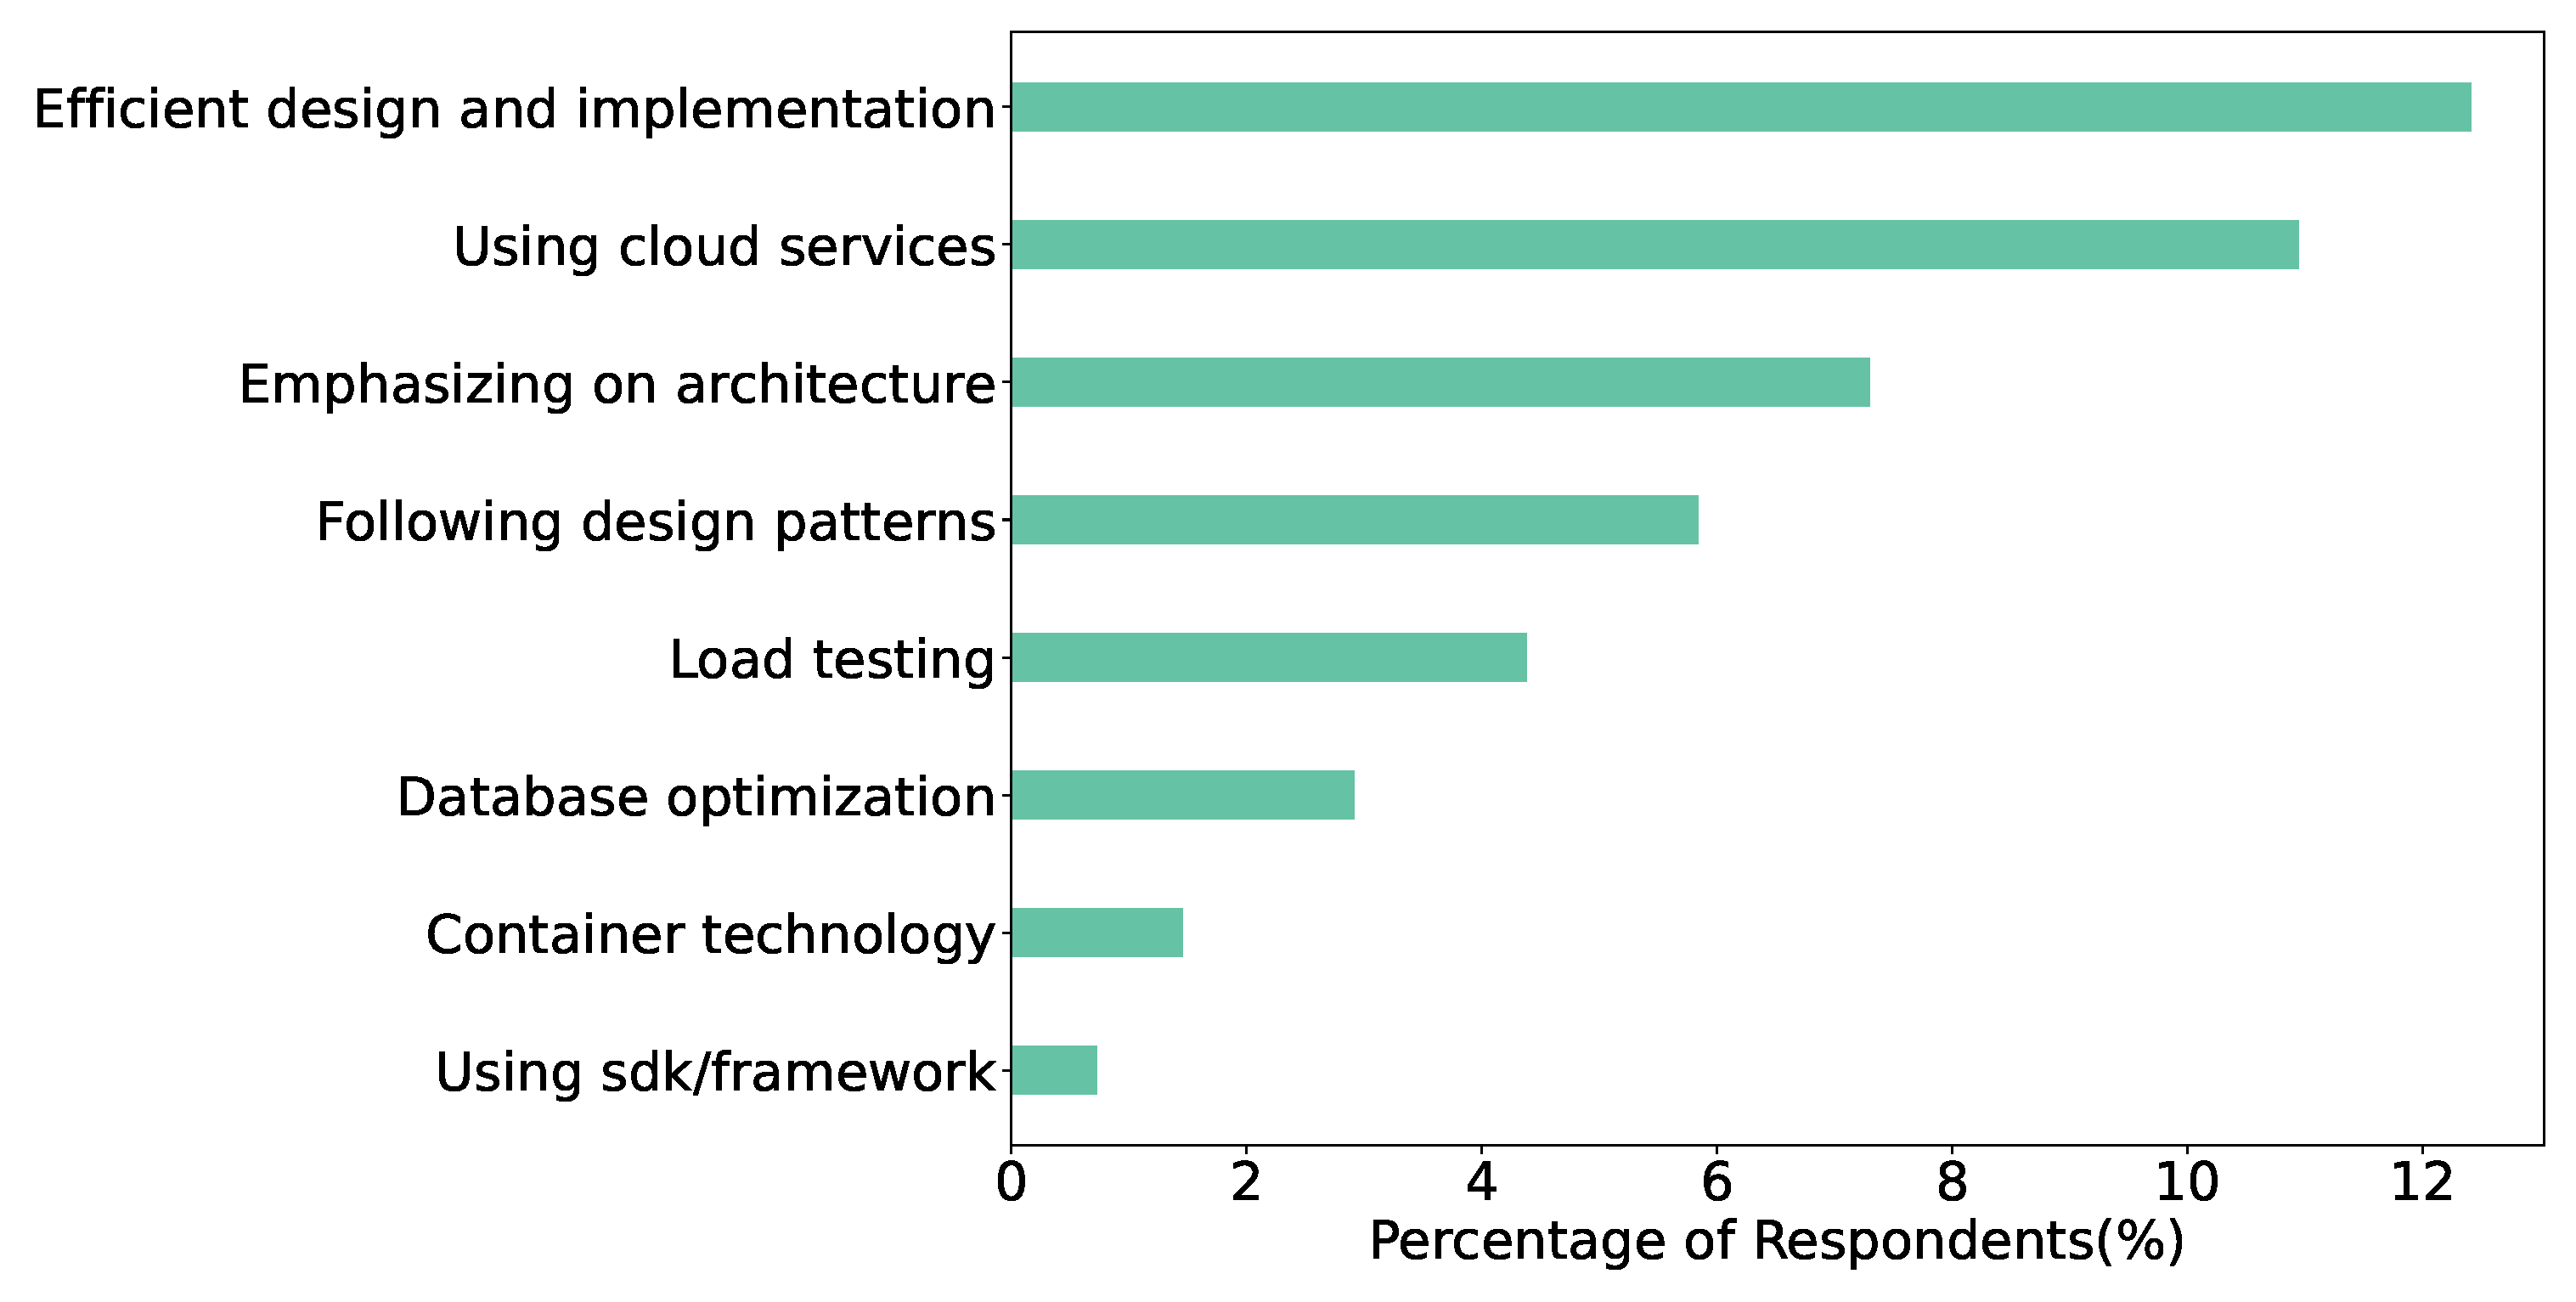
\includegraphics[scale=0.28]{Figures/Scalability.eps} 
\caption{Measures to ensure scalability of products}
\label{fig:Measures to ensure scalability}
\end{figure}
\hfill\\
 Software scalability defines the ability to scale up a solution. Issues with little importance can impede scaling up. Thus proper measures should be taken from design stage to ensure the scalability of system. Recent days the cloud services offer tools to accomodate custom reactive scaling strategies. Thus, it has become easier to ensure scalability using cloud services \citep{Falatah2014}. Our results  also follows the world trend, usage of cloud services has placed 2\textsuperscript{nd} in terms popularity of scalability measures in SE industry of Bangladesh.
\begin{enumerate}
    
    \item \textbf{Following Certain Design Patterns}: There are some design patterns which inherently help us in time of scaling. 5.84\% people think that Following these design patterns will be of great use.
    \surveyquote{Following certain design patterns}{8}
    
    \item \textbf{Based on Framework}: Modern frameworks ensures scalability by default. 0.73\% respondents solely depends on framework for scalability.
    \surveyquote{following flexible framework which allows better scalability}{14}
    
    
    \item \textbf{Container Technology}: Container technologies includes docker, Kubernetes which ensures OS level virtualization. By standardizing the system, container technologies eases the scaling of an infrastructure.
    \surveyquote{We used Docker technology}{85}
    
    \item \textbf{Database Optimization}: Database optimization includes sharding, clustering, indexing and scaling. 10.3\% respondents optimize database to scale their system.
    \surveyquote{Besides scaling horizontally, database scaling is performed by partitioning tables, along with multi-threaded implementations}{85}
    
    \item \textbf{Efficient Design and Implementation}: 12.41\% respondents emphasizes on  the design and implementation of a scalable architecture.
    \surveyquote{During implementation we always keep in mind about the scaling factor}{40}
    
    \item \textbf{Emphasizing on architecture}: 7.3\% respondents emphasized on architecture. It is mostly micro-service architecture which they use to ensure scalability.
    \surveyquote{We follow the micro-service architecture. In a nutshell, we scale up the module vertically which is necessary. We use docker along with Jenkins for automatic deployments and scaling.}{10}
    
    \item \textbf{Load Testing}: Load testing can be used to check the scalability of a system. 4.38\% respondents use load test to check wheather their system is scalable or not.
    \surveyquote{through load testing and load simulation.}{35}
    
    \item \textbf{Using Cloud Services}: 10.95\% user depends on Clod services like AWS and Azure  for the scalability of system. Modern features like elastic load balancing and  auto- scaling makes it easy to ensure scalability.
    \surveyquote{Using AWS Elastic Load Balancer}{28}
    
    
    
\end{enumerate}
